%% Author: Mark weinreuter

\documentclass[12pt,a4paper,oneside,ngerman]{scrbook}

\usepackage[utf8]{inputenc}
\usepackage{fancyhdr} % Required for custom headers
\usepackage{lastpage} % Required to determine the last page for the footer
\usepackage{extramarks} % Required for headers and footers
\usepackage[usenames,dvipsnames]{color} % Required for custom colors
\usepackage{graphicx} % Required to insert images
\usepackage{listings} % Required for insertion of code
\usepackage{courier} % Required for the courier font
\usepackage{lipsum} % Used for inserting dummy 'Lorem ipsum' text into the template

% Set up the header and footer
\pagestyle{fancy}

%\chead{\hmwkTitle} % Top center head
\rhead{\hmwkAuthorName} % Top left header
%\rfoot{Seite\ \thepage\ von\ \protect\pageref{LastPage}} % Bottom right footer
\renewcommand\headrulewidth{0.4pt} % Size of the header rule
\renewcommand\footrulewidth{0.4pt} % Size of the footer rule

\setlength\parindent{0pt} % Removes all indentation from paragraphs
\setcounter{chapter}{1}

%----------------------------------------------------------------------------------------
%	CODE INCLUSION CONFIGURATION
%----------------------------------------------------------------------------------------

\definecolor{MyDarkGreen}{rgb}{0.0,0.5,0.0} % This is the color used for comments
\definecolor{DarkGreen}{rgb}{0.0,0.4,0.0} % This is the color used for comments

\lstloadlanguages{Python} 
\lstdefinestyle{line_numbers} {numbers=left, stepnumber=1, numberstyle=\tiny, numbersep=10pt}
\lstdefinestyle{MyFrame}{backgroundcolor=\color{yellow},frame=shadowbox}
\lstdefinestyle{Pseudo} {language=Python,style=MyFrame,frame=lines}
\lstdefinestyle{Python} {language=Python,style=line_numbers,frame=lines}
\lstdefinestyle{Output} {language=Python,style=line_numbers,frame=lines}

\lstset{language=Python, % Use Perl in this example
        frame=single, % Single frame around code
        basicstyle=\small\ttfamily, % Use small true type font
        keywordstyle=[1]\color{Blue}\bf, % Perl functions bold and blue
        keywordstyle=[2]\color{DarkGreen}, % Perl function arguments purple
        keywordstyle=[3]\color{Blue}\underbar, % Custom functions underlined and blue
        identifierstyle=, % Nothing special about identifiers                                         
        commentstyle=\usefont{T1}{pcr}{m}{sl}\color{MyDarkGreen}\small, % Comments small dark green courier font
        captionpos=b,
        stringstyle=\color{Purple}, % Strings are purple
        showstringspaces=false, % Don't put marks in string spaces
        tabsize=4, % 5 spaces per tab
        %
        % Python Keywords, etc die nicht markiert sind
        morekeywords={False, True},
        %
        % Benutzerdefiniertes Zeug
        morekeywords=[2]{Spiel, Polygon, Linien, Rechteck, Schrift},
        %
        % Noch mehr benutzerdefiniertes Zeug (andere Farbe)
        morekeywords=[3]{test},
       	%
        morecomment=[l][\color{Blue}]{...}, % Line continuation (...) like blue comment
        numbers=left, % Line numbers on left
        firstnumber=1, % Line numbers start with line 1
        numberstyle=\tiny\color{Blue}, % Line numbers are blue and small
        stepnumber=5 % Line numbers go in steps of 5
}

%Für Umlaute, etc
\lstset{literate=%
	{Ö}{{\"O}}1
	{Ä}{{\"A}}1
	{Ü}{{\"U}}1
	{ß}{{\ss}}1
	{ü}{{\"u}}1
	{ä}{{\"a}}1
	{ö}{{\"o}}1
	{~}{{\textasciitilde}}1
}

\newcommand{\code}[1]{
	\begin{ttfamily}#1\end{ttfamily}
}

%----------------------------------------------------------------------------------------
%	NAME AND CLASS SECTION
%----------------------------------------------------------------------------------------

\newcommand{\hmwkTitle}{if-Abfragen}
\newcommand{\hmwkClass}{Basics:\space} 
\newcommand{\hmwkAuthorName}{CoderDojoKa}

%----------------------------------------------------------------------------------------

\begin{document}

\begin{center}
	{\huge \hmwkTitle}
\end{center}

\section{Entscheidungen und Bedingungen}
An vielen Stellen im täglichen Leben, sowie auch beim Programmieren müssen Entscheidungen getroffen werden:
"Soll ich früher aufstehen, um ihn Ruhe zu früchstücken oder lass ich das Frühstück ausfallen, damit ich länger schlafen kann?"
	
Um nun abends den Wecker zu stellen muss man sich Folgendes überlegen und ausführen:

\begin{lstlisting}[style=Pseudo]
Falls <Will ich frühstücken?>:
	stelle_wecker(6)
Ansonsten:
	stelle_wecker(7)
\end{lstlisting}

Die Weckzeit ist also abhängig von der Bedingung: "Will ich frühstücken?".

\paragraph{Bedingung} Eine Bedingung beim Programmieren ist eine Aussage oder ein Ausdruck,
die mit "Ja" oder "Nein" zu beantworten ist. Komplizierte Antworten gibt es nicht! Eine Antwort
muss immer "Ja" oder "Nein" sein, "Vielleicht" oder "Morgen" sind nicht erlaubt.
\\
Um genau zu sein heißen diese Werte beim Programmieren meistens \code{True} (engl. für "Wahr") und \code{False} (engl. für "Falsch").
\\
Vielleicht stellst Du Dir jetzt die Frage, wie eine Bedingung zu formulieren ist, da "Will ich frühstücken?" für Menschen einfach zu verstehen ist, für einen Computer allerdings nicht.

\paragraph{Die einfachste Bedinung} ist \code{True}("Wahr") oder \code{False} ("Falsch") zu schreiben.
\begin{lstlisting}[style=Pseudo]
Falls <Wahr>:
	sage("Die Bedingung ist wahr")
\end{lstlisting}
Zugebenermaßen ist dies nicht sinnvoll, da man in dem obigen Beispiel die Bedingung einfach weglassen kann.
	
\paragraph{Vergleichsoperationen} sind eine Möglichkeit um Bedingungen zu beschreiben. Wie in der Schule können z.B. Operationen wie \code{>} (größer), \code{<} (kleiner),\code{>=} (größer gleich), \code{<=} (kleiner gleich) verwendet werden um Zahlen zu vergleichen.
\\
\\
Ein Ausdruck wie \code{30 > 20} ergibt \code{True} und \code{30 < 20} ergibt \code{False.} Diese können also als Bedingung verwendet werden kann.

\begin{lstlisting}[style=Pseudo]
# 'alter' ist eine zuvor definierte Variable
Falls alter > 10:
	sage("Du bist älter als 10")
\end{lstlisting}

\clearpage

\begin{table}[t,clr]
	\begin{center}
	\begin{tabular}{|l|l|l|l|}
		\hline
		Operation		& Befehl		   	& Beispiel			 				& Ausgabe\\ \hline\hline
		Größer         	& \textgreater  	& 20 \textgreater\space20  			& Falsch \\ \hline
		Größer Gleich  	& \textgreater= 	& 20 \textgreater= 20 				& Wahr   \\ \hline
		Kleiner        	& \textless     	& 10 \textless\space30				& Wahr   \\ \hline
		Kleiner Gleich	& \textless=    	& 10 \textless= 25	    			& Wahr   \\ \hline
		Gleichheit    	& ==            	& 10 == 10	            			& Wahr   \\ \hline
		Ungleichheit  	& !=            	& 10 != 10            				& Falsch \\ \hline
	\end{tabular}
	\caption{Vorhandene Vergleichsoperationen}
	\end{center}
\end{table}

\section{Aufgaben}
\begin{itemize}
	\item Was (\code{True} oder \code{False}) ergeben die folgenden Ausdrücke jeweils:
	\begin{itemize}
		\item 10 \textless\space 12:
		\item 12 \textless\space 10
		\item 15 != 15
		\item 20 \textgreater= 15
		\item 12 == 12
	\end{itemize}
	\item In der Variablen \code{Schuhgröße} steht die Schuhgröße einer Person.
	\\
	Schreibe eine Falls-Ansonsten-Abfrage, die ausgibt (benutze "sage"), ob diese Person große Füße hat oder nicht. Große Füße bedeutet, dass die Schuhgröße größer als 42 ist.
\end{itemize}

\clearpage

\section{if-Abfrage (Falls-Abfrage)} Bisher haben wir in den Beispielen keinen 'echten' Code verwendet. Dies wollen wir jetzt ändern.
Eine "Falls"-Abfrage sieht in Python so aus:

\begin{lstlisting}[style=Python, caption='Kleiner'-Vergleich mit einer Variablen]
# 'wert' ist eine zuvor definierte beliebige Zahl-Varible
if wert < 10:
	print("Kleiner 10.")
	
print("Nach if-Abfrage.")
\end{lstlisting}

Dazu schreibt man \code{if} (engl. für "falls), dann die Bedingung gefolgt von einem Doppelpunkt ':'. Darunter eine oder mehrere eingerückte Zeilen.
\\
Die Einrückung (mit 4 Leerzeichen oder Tabulator-Taste) bedeutet, dass alles was eingerückt ist \textbf{genau dann} ausgeführt wird, wenn die Bedingung wahr ist.
\\
\\
Führt man dies nun aus mit den Werten \code{wert = 5} und \code{wert = 15} aus, verhält sich die Ausgabe unterschiedlich:
\begin{lstlisting}[style=Output, caption=Ausgabe für kleineren Wert]
# wert = 5
Kleiner 10.
Nach if-Abfrage.
\end{lstlisting}


\begin{lstlisting}[style=Output, caption=Beispiel Ausgabe für größeren Wert]
# wert = 15
Nach if-Abfrage.
\end{lstlisting}

Man sieht an den Beispielen, dass "Kleiner 10." nur dann ausgegeben wird, wenn der Wert kleiner als 10 ist. Die nichteingerückte Zeile darunter wird in beiden Fällen ausgeführt und dies führt dazu, dass "Nach if-Abfrage." immer ausgeben wird.


\paragraph{Falls-Ansonsten-Abfrage (if-else-Abfrage)} Ist die Bedingung in der "Falls"-Abfrage falsch, so kann eine "Ansonsten"-Abfrage (engl. "else") hinzugefügt werden, die \textbf{genau dann} ausgeführt wird, wenn die Bedingung falsch ist.

\begin{lstlisting}[style=Python, caption='Kleiner'-Vergleich mit if-else-Abfrage]
# 'wert' ist eine zuvor definierte beliebige Zahl-Varible
if wert < 10:
	print("Kleiner 10.")
else:
	print("Größer oder gleich 10.")

print("Nach if-Abfrage.")
\end{lstlisting}
Führt man dies nun aus mit den Werten \code{wert = 5} und \code{wert = 15} aus, verhält sich die Ausgabe wie folgt:
\begin{lstlisting}[style=Output, caption=Ausgabe für kleineren Wert]
# wert = 5
Kleiner 10.
Nach if-Abfrage.
\end{lstlisting}

\begin{lstlisting}[style=Output, caption=Beispiel Ausgabe für größeren Wert]
# wert = 15
Größer oder gleich 10.
Nach if-Abfrage.
\end{lstlisting}

\paragraph{In Scratch} würde das obige Beispiel dann so aussehen:
\\
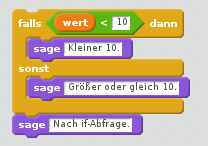
\includegraphics[scale=1]{scratch_if_else}
\\
Man sieht hier sehr schön die Einrückungen der "sage"-Blöcke, während der grüne sptize Block die Bedingung darstellt.



\section{Aufgaben}
\begin{itemize}
	\item Du hast eine Variable 'zufall', die einen zufälligen Wert hat:
	\begin{lstlisting}[caption=Python Code für eine zufällige Variable zwischen 1-100]
import random
zufall = random.randint(1, 100)
	\end{lstlisting}
	Schreibe eine if-else Abfrage die bestimmt, ob der Wert der Variablen größer oder gleich 50 ist oder nicht. Gib dies dann mithilfe des print() aus.
\end{itemize}

\end{document}